%sección IV
\section{Método de revisión}
Con el fin de alcanzar los objetivos propuestos para este articulo, se usó un acercamiento metodológico basado en que siguen Sepúlveda et al [Referencia del articulo de Sepúlveda] para construir un estudio de mapeo sistemático (SMS por sus siglas en inglés) basado en evidencia.

De acuerdo a los estudios [Sepulveda's article citations 16 and 17], es posible usar una combinación de estrategias de búsqueda para crear un SMS. Debido a esto, se ha decidido mezclar dos estrategias de búsqueda, una automática y la otra manual, para el mapeo sistemático propuesto en este articulo. También, se ha usado la metodología propuesta por Ali et al [Sepulveda's article citations 18] como un ejemplo.

Por ultimo, se ha soportado el proceso de construcción de este SMS con la ayuda del software SMS-Builder. Este software es una aplicación web que se creó para ayudar a los investigadores a seguir el proceso de construcción de una adaptación del SMS propuesto por [Sepulveda's article citations 14], que cubre seis fases del proceso de construcción del mapeo sistemático 1) Planeación, 2) Búsqueda de estudios, 3) Análisis de calidad, 4) Recolección de datos, 5) Clasificación y análisis de estudios, 6) Resultados. Ver Figura \ref{figure:Stages}. Para el estudio propuesto en este articulo, se usó SMS-Builder para guardar, procesar, analizar y evaluar los estudios a ser incluidos en el SMS [Sepulveda's article citations 19]. La herramienta puede ser encontrada en GitHub como software libre bajo la licencia GNU/GPL v3 en el siguiente link: https://github.com/grid-uq/sms-builder [Sepulveda's article citations 19].

\begin{figure}[htbp]
	\centering
	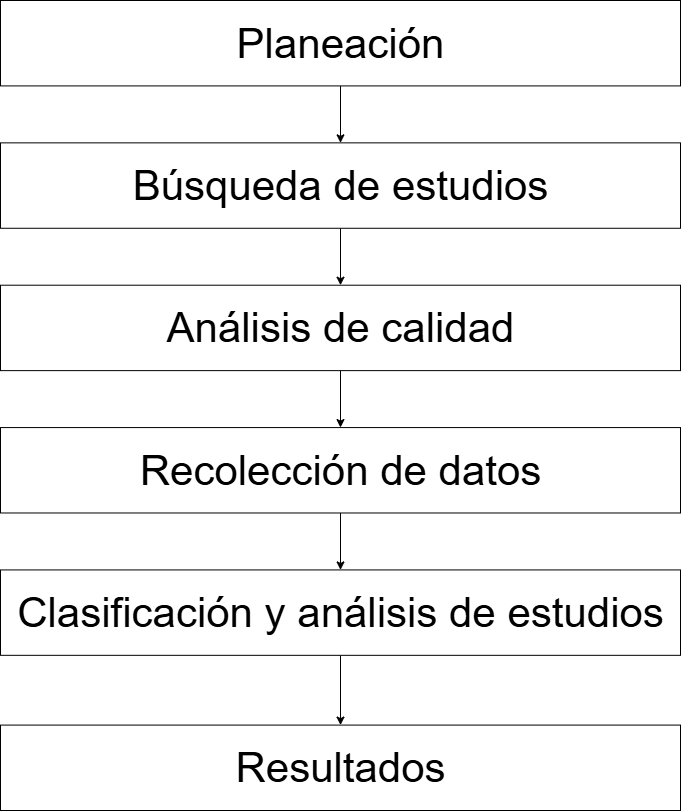
\includegraphics[width=0.9\linewidth]{resources/figures/sms-Etapas.drawio.png}
	\caption{Etapas del proceso de construcción de un SMS}
	\label{figure:Stages}
\end{figure}

% ETAPAS
%subsección 4.1 
\subsection{Planeación}
En esta etapa, se estableció el propósito general de la investigación y se definieron las metas, así como las preguntas de investigación, métricas, criterios de clasificación, criterios de inclusión/exclusión y criterios de calidad de los estudios. Ver Figura~\ref{fig:etapa1}.

\begin{figure*}[tbp]
    \centering
    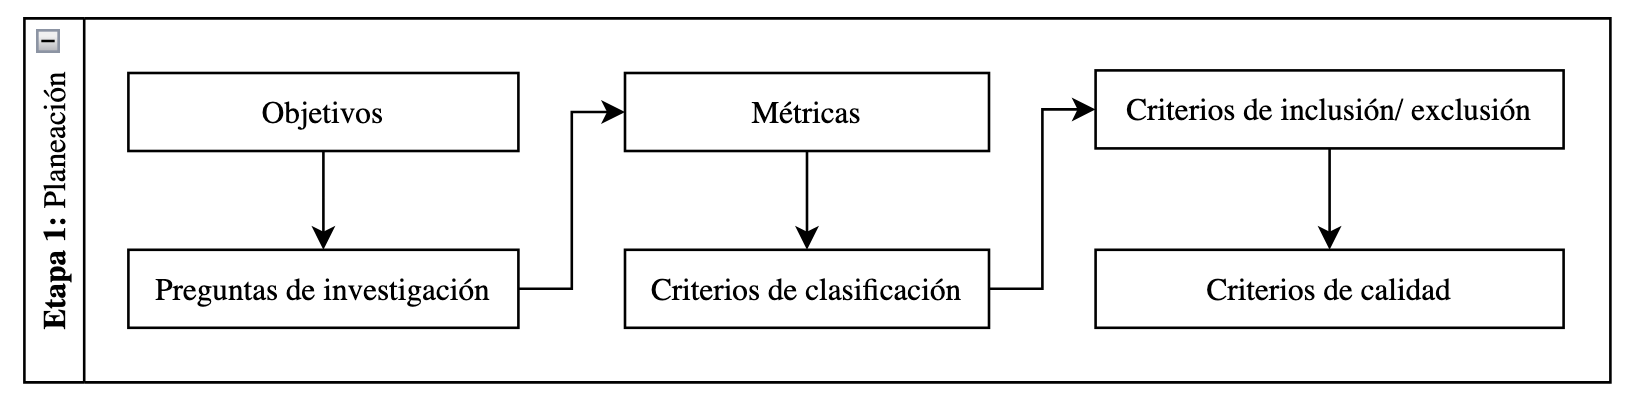
\includegraphics[width=0.8\textwidth]{resources/images/planeacion/etapa1.png}
    \caption{Composición de la etapa de planeación}\label{fig:etapa1}
\end{figure*}

\subsubsection{Objetivos}
\mbox{}\\
Teniendo en cuenta los aspectos descritos en la sección de motivación, se definieron 2 metas generales para la revisión sistemática de la literatura que se presentan en el cuadro~\ref{tab:metas}.

\begin{table}[htbp]
    \centering
    \begin{tabular}{>{\centering\arraybackslash}m{1cm} >{\arraybackslash}m{7cm}}
        \hline
        \textbf{Goal} & \textbf{Description} \\
        \hline
        M1 & Identificar trabajos relacionados con VBC en proyectos de docencia, investigación y extensión. \\
        \\
        M2 & Clasificar trabajos relacionados con VBC en los dominios de desarrollo de software, pensamiento computacional, computación paralela, análisis de datos, inteligencia artificial, redes computacionales, infraestructura de TI, HPC, entre otros. \\
        
        \hline
    \end{tabular}
    \caption{Metas del estudio}\label{tab:metas}
\end{table}





\subsubsection{Pregunta de investigación}
\mbox{}\\

\begin{table}[tbp]
    \scriptsize % reduce tamaño del texto
    \centering
    \renewcommand{\arraystretch}{1.3}
    \begin{tabularx}{\columnwidth}{>{\centering\arraybackslash}m{0.18\columnwidth} >{\RaggedRight\arraybackslash}X}
        \hline
        \textbf{Aspecto} & \textbf{Descripción} \\
        \hline
        Población & Trabajos relacionados con la VBC aplicadas en diversos dominios de TI con un énfasis en la educación, investigación y extensión. \\
        Intervención & Identificación y clasificación de los trabajos en VBC en los dominios de TI establecidos. \\
        Comparación & 
        1. Se comparan los proyectos que han hecho uso de la VBC para determinar cuáles han tenido mayor tasa de éxito expresado por los autores en cada dominio de TI. \newline
        2. Se analiza el impacto de la VBC en proyectos de docencia, investigación y extensión en comparación con otras soluciones tecnológicas. \\
        Salida & Estructura de clasificación de los trabajos relacionados con las VBC en cada dominio de TI que han impactado en proyectos de docencia, investigación y extensión. \\
        Contexto & Docencia, investigación y extensión con apropiación de los dominios de TI en forma de VBC. \\
        \hline
    \end{tabularx}
    \caption{Aspectos del modelo PICOC}\label{tab:PICOC}
\end{table}

\begin{table*}[!t]
\centering

\renewcommand{\arraystretch}{1.4}
\begin{tabularx}{\textwidth}{>{\centering\arraybackslash}m{0.05\textwidth} >{\centering\arraybackslash}m{0.05\textwidth} >{\RaggedRight\arraybackslash}X >{\RaggedRight\arraybackslash}X}
\toprule
\textbf{Meta} & \textbf{Pregunta} & \textbf{Descripción} & \textbf{Motivación} \\
\midrule
G1 & Q1 & ¿Cuáles son los trabajos relacionados con tecnologías de virtualización basadas en contenedores (VBC) que podrían impactar positivamente proyectos de docencia, investigación y extensión? & La transversalidad que ofrece la VBC, gracias a su reproducibilidad de entornos, permite estimular diferentes aristas de la sociedad. Su naturaleza facilita el transporte de soluciones de TI entre diferentes entornos, generando que una innovación en cualquier dominio social impacte directamente en otro. \\
\midrule
G2 & Q2 & ¿Cuáles son los principales trabajos relacionados con las tecnologías de virtualización basadas en contenedores (VBC) que podrían contribuir en los diversos dominios de TI, entre los que pueden ser desarrollo de software, pensamiento computacional, computación paralela, análisis de datos, inteligencia artificial, redes computacionales, infraestructura de TI, HPC, entre otros? & Se busca proporcionar una base sólida para investigadores, docentes y profesionales interesados en comprender el estado del arte actual en relación con las VBC, además del alcance y las aplicaciones de estos trabajos sin necesidad de un análisis profundo. \\
\bottomrule
\end{tabularx}
\caption{Preguntas de investigación y su motivación}
\label{tab:preguntas}
\end{table*}

Este modelo permite establecer los aspectos de ``Población'', ``Intervención'', ``Comparación'', ``Salida'' y ``Contexto'' que sirven para situar el trabajo a realizar. Ver cuadro~\ref{tab:PICOC}. \\
\\
Teniendo en cuenta el modelo PICOC, se definieron las preguntas de investigación. Ver cuadro~\ref{tab:preguntas}.



\subsubsection{Métricas}
\mbox{}\\
Texto por agregar...

\subsubsection{Tópicos de investigación}
\mbox{}\\
Texto por agregar...

\subsubsection{Criterios de inclusión y exclusión}
\mbox{}\\
Texto por agregar...

\subsubsection{Criterios de calidad}
\mbox{}\\
Texto por agregar...

%subsección 4.2
% subseccion 4.2
\subsection{Etapa 2: Búsqueda de Estudios}
Esta etapa presenta la estrategia de búsqueda usada en la revisión sistemática de la literatura. Esta estrategia se describe en detalle en las subsecciones~\ref{subsubsec:Definiendo la Estrategia de Busqueda} -- \ref{subsubsec:resultados-busqueda}. Ver figura~\ref{fig:etapa2}.

\begin{figure*}[tbp]
    \centering
    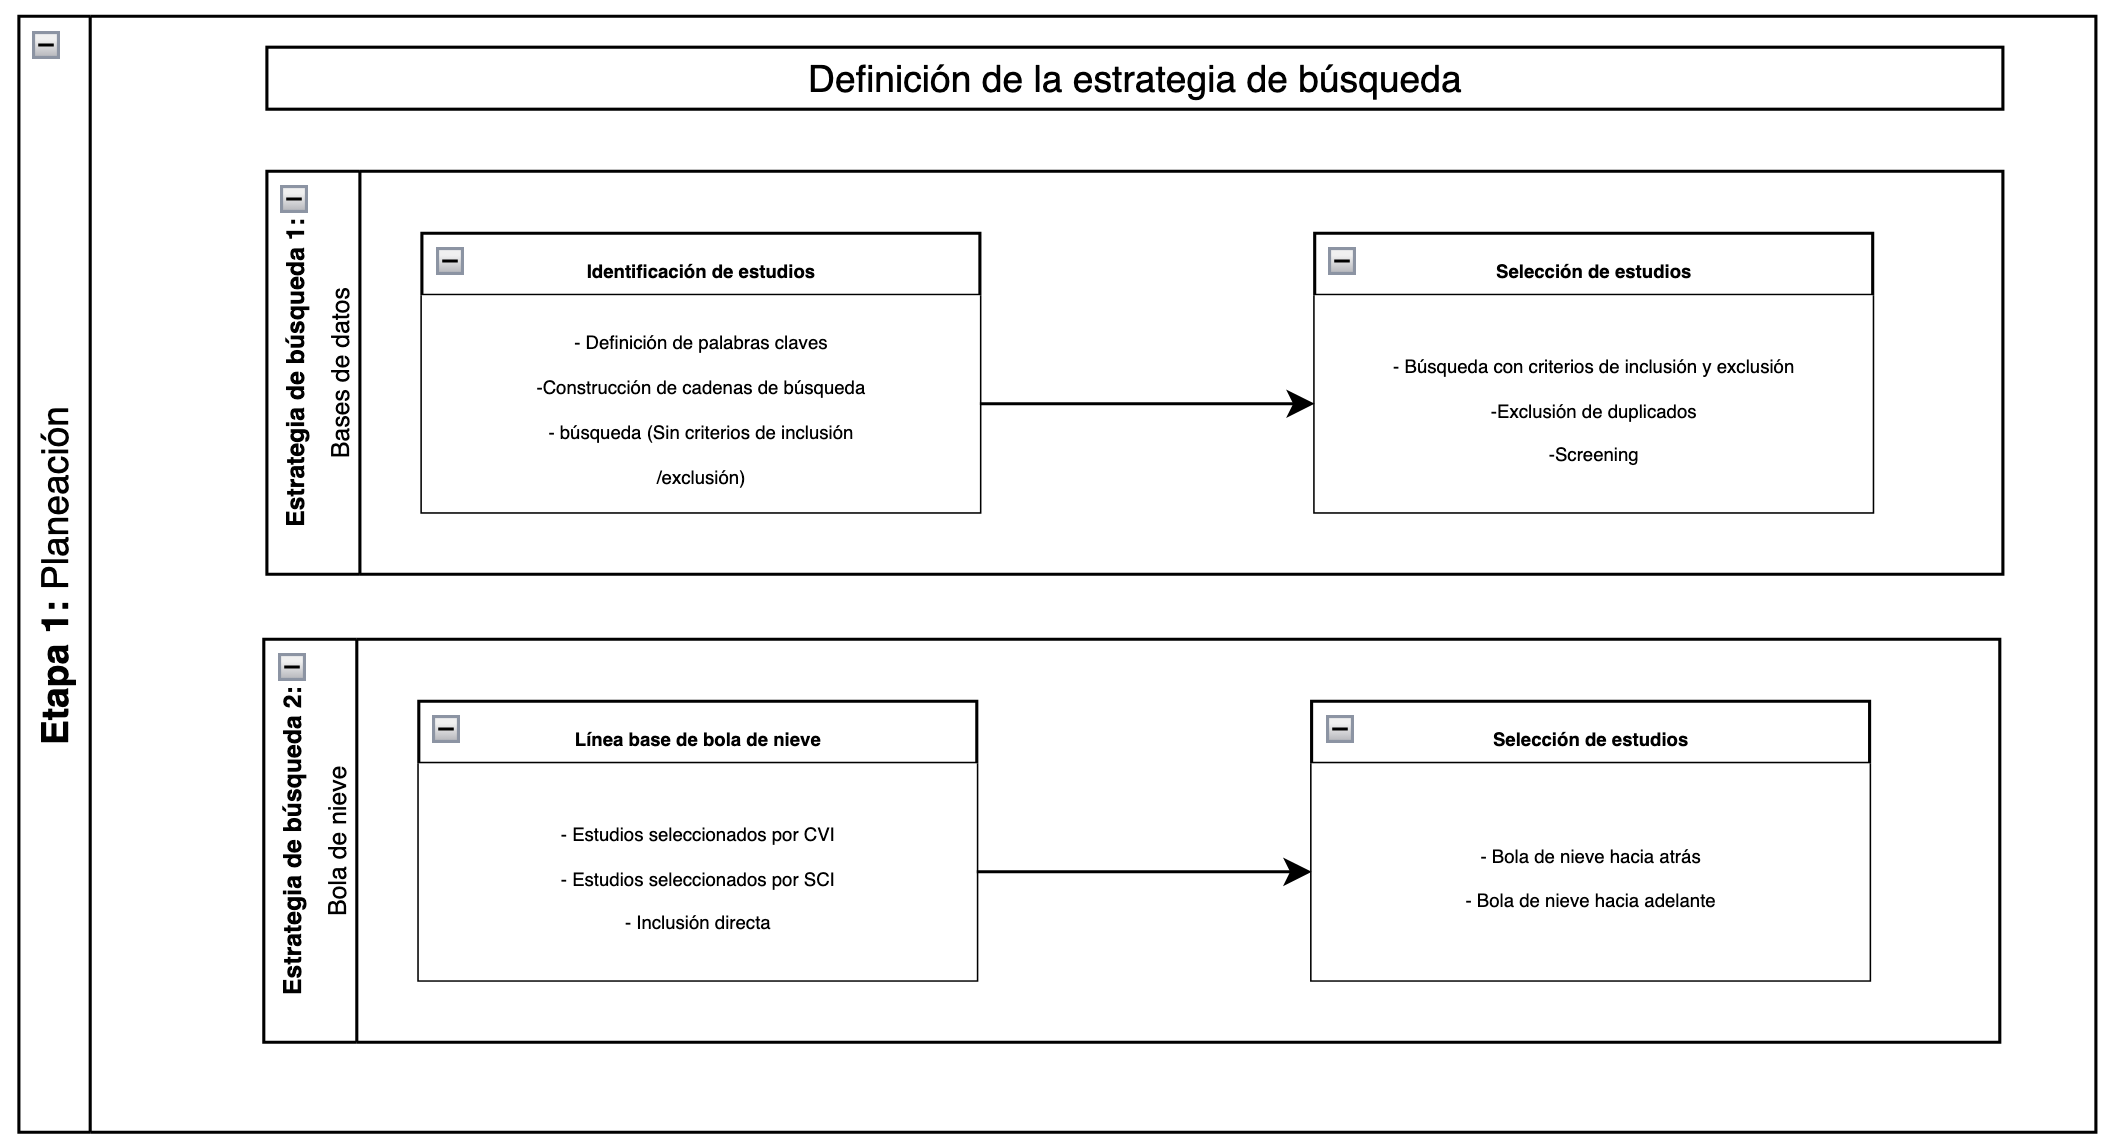
\includegraphics[width=0.8\textwidth]{resources/images/planeacion/estrategias-busqueda.png}
    \caption{Composición de la etapa de búsqueda de estudios}\label{fig:etapa2}
\end{figure*}
\mbox{}\\

%sub-subseccion 4.2.1 
\subsubsection{Definiendo la Estrategia de Búsqueda}\label{subsubsec:Definiendo la Estrategia de Busqueda}
\mbox{}\\
% Content for 4.2.1
Para la construcción de esta revisión de la literatura, se usó un enfoque híbrido. Con este enfoque se busca obtener mayor volumen de artículos indexados y con diferentes origenes. más allá de los proporcionados por las bases de datos.
En este sentido, se combinaron dos estrategias de búsqueda. La primer estrategia es la búsqueda en bases de datos y consiste en realizar una cadena de búsqueda automatizada en bases de datos académicas.~\cite{jalali2012systematic}.
La segunda estrategia es la denominada ``Bola de Nieve'' (Snowballing) y consiste en la búsqueda manual de artículos a partir de un conjunto base de artículos usando las referencias y las citas de los mismos. Esta estrategia se basa en la premisa de que los artículos relevantes citan otros artículos relevantes y, por lo tanto, permite encontrar artículos que no están indexados en las bases de datos académicas.~\cite{jalali2012systematic} y \cite{goodman1961snowball}.
\mbox{}\\
%sub-subseccion 4.2.2

\subsubsection{Estrategia de Búsqueda 1: Bases de Datos}
\mbox{}\\
Esta estrategia consta de 2 componentes. El primer componente es denominado ``Identificación de estudios''. Esto se enfoca en definir las palabras clave para construir las cadenas de búsqueda que conducen a completar las búsquedas en las bases de datos académicas.
El segundo componente es llamado ``Selección de estudios''. Se enfoca en aplicar varios criterios para refinar la búsqueda de resultados de estudios y así obtener el mayor valor del proceso de búsqueda. \\ \\

\begin{itemize}
    \item \textbf{Identificación de estudios:} En búsqueda de la viabilidad del estudio y por acuerdo de los autores, se limitó la búsqueda a cinco bases de datos académicas: \textit{ACM}, \textit{IEEE Xplore}, \textit{Springer}, \textit{Science Direct} y \textit{Taylor and Francis}. En esta parte del proceso es necesario establecer las palabras claves definidas antes y construir las cadenas de búsqueda específica para cada base de datos. Nuevamente se usó el modelo PICOC como guía metodológica para identificar términos claves o frases completas que se relacionan con las tecnologías de virtualización basadas en contenedores. En la construcción de estas cadenas de búsqueda se usaron sinónimos para ampliar el espectro de resultados. (Ver cuadro~\ref{tab:palabras-clave}).\\ 
    Las principales palabras clave identificadas fueron: \textit{Container-based virtualization}, \textit{Education}, \textit{Research}, \textit{Industry}. Para ampliar y refinar los resultados se usaron operadores booleanos como \textit{AND} y \textit{OR}. Además, se usaron comillas para buscar frases completas y paréntesis para agrupar términos relacionados. Finalmente, el conjunto de palabras clave seleccionadas para construir las cadenas de búsqueda se presenta en el cuadro~\ref{tab:keywords}.\\
    Para dirigir la búsqueda hacia la intercepción de los dominios de TI y la VBC se usó el operador booleano \textit{AND}. Una vez identificadas las palabras clave, se procedió con la construcción de las cadenas de búsqueda para cada base de datos, usando un proceso iterativo. El proceso de construcción de las cadenas de búsqueda consitió en realizar un proceso heúristico con las palabras clave, sinónimos y conceptos relacionados, haciendo uso de conjunciones y disyunciones conforme a las reglas de cada base de datos.\\ 
    Así, estas cadenas de búsqueda varían de acuerdo con las reglas de cada base de datos. Ver cuadro~\ref{tab:cadenas-busqueda}.\\

\end{itemize}

\begin{table}[tbp]
    \scriptsize % reduce tamaño del texto
    \centering
    \renewcommand{\arraystretch}{1.3}
    \begin{tabularx}{\columnwidth}{>{\centering\arraybackslash}m{0.18\columnwidth} >{\RaggedRight\arraybackslash}X}
        \hline
        \textbf{Aspecto} & \textbf{Descripción} \\
        \hline
        Población & VBC, Dominios de TI, Educación, Investigación, Extensión \\
        Intervención & Identificación, Clasificación \\
        Comparación & Tasa de éxito, Evidencia de uso \\
        Salida & Clasificación de trabajos relacionados con VBC en cada dominio de TI \\
        Contexto & Docencia, Investigación, Extensión \\
        \hline
    \end{tabularx}
    \caption{Palabras clave identificadas usando el modelo PICOC}\label{tab:palabras-clave}
\end{table}

\begin{table}[tbp]
    \scriptsize % reduce tamaño del texto
    \centering
    \renewcommand{\arraystretch}{1.3}
    \begin{tabularx}{\columnwidth}{>{\centering\arraybackslash}m{0.18\columnwidth} >{\RaggedRight\arraybackslash}X}
        \hline
        \textbf{Palabras clave} & \textbf{Sinónimos} \\
        \hline
        Container-based virtualization & Application virtualization, Docker, Lightweight Virtualization \\
        Education & Education System, Education Development, Higher Education \\
        Research & Research Group, Research Proposal \\
        Industry & IT Services, Technology Infrastructure, Cloud Computing \\
        \hline
    \end{tabularx}
    \caption{Palabras clave para la búsqueda en base de datos}\label{tab:keywords}
\end{table}




\newcolumntype{P}[1]{>{\raggedright\arraybackslash}p{#1}}

\begin{sidewaystable*}[htbp]
\centering
\scriptsize
\renewcommand{\arraystretch}{1.5}
\caption{Cadenas de búsqueda por dominio y base de datos}
\label{tab:cadenas-busqueda}
\begin{adjustbox}{max width=\textwidth}
\begin{tabular}{|P{0.18\linewidth}|P{0.20\linewidth}|P{0.20\linewidth}|P{0.20\linewidth}|P{0.20\linewidth}|}
\hline
\textbf{Dominio / Base de Datos} & \textbf{ACM Digital Library} & \textbf{IEEE Xplore} & \textbf{ScienceDirect} & \textbf{SpringerLink} \\
\hline

\textbf{Educación AND VBC} 
& \tiny (Title:("Container-based virtualization" OR "Application virtualization" OR "Docker" OR "Lightweight Virtualization") AND Title:("Education" OR "Education System" OR "Education Development" OR "Higher Education")) OR (Abstract:("Container-based virtualization" OR "Application virtualization" OR "Docker" OR "Lightweight Virtualization") AND Abstract:("Education" OR "Education System" OR "Education Development" OR "Higher Education")) OR (Keyword:("Container-based virtualization" OR "Application virtualization" OR "Docker" OR "Lightweight Virtualization") AND Keyword:("Education" OR "Education System" OR "Education Development" OR "Higher Education"))
& ("container-based virtualization") AND ("education" OR "educational use") 
& ("container-based virtualization" AND "education") 
& ("container-based virtualization" OR docker) AND ("education" OR "learning environment") \\
\hline

\textbf{Investigación AND VBC} 
& \tiny (Title:("Container-based virtualization" OR "Application virtualization" OR "Docker" OR "Lightweight Virtualization") AND Title:("Research" OR "Research Group" OR "Research Proposal")) OR (Abstract:("Container-based virtualization" OR "Application virtualization" OR "Docker" OR "Lightweight Virtualization") AND Abstract:("Research" OR "Research Group" OR "Research Proposal")) OR (Keyword:("Container-based virtualization" OR "Application virtualization" OR "Docker" OR "Lightweight Virtualization") AND Keyword:("Research" OR "Research Group" OR "Research Proposal"))
& ("container-based virtualization") AND ("scientific research" OR "research proposal") 
& ("container-based virtualization" AND "research") 
& ("container-based virtualization" OR docker) AND ("research" OR "experiments") \\
\hline

\textbf{Industria AND VBC} 
& \tiny (Title:("Container-based virtualization" OR "Application virtualization" OR "Docker" OR "Lightweight Virtualization") AND Title:("Industry" OR "IT Services" OR "Technology Infrastructure" OR "Cloud Computing")) OR (Abstract:("Container-based virtualization" OR "Application virtualization" OR "Docker" OR "Lightweight Virtualization") AND Abstract:("Industry" OR "IT Services" OR "Technology Infrastructure" OR "Cloud Computing")) OR (Keyword:("Container-based virtualization" OR "Application virtualization" OR "Docker" OR "Lightweight Virtualization") AND Keyword:("Industry" OR "IT Services" OR "Technology Infrastructure" OR "Cloud Computing"))
& ("container-based virtualization") AND ("IT industry" OR "enterprise deployment") 
& ("container-based virtualization" AND "industry") 
& ("container-based virtualization" OR docker) AND ("industry" OR "production environment") \\
\hline

\textbf{Taylor and Francis} 
& ("container-based virtualization") AND ("higher education" OR "education system") 
& ("container-based virtualization") AND ("research group" OR "academic research") 
& ("container-based virtualization") AND ("IT services" OR "technology infrastructure") 
& --- \\
\hline

\end{tabular}
\end{adjustbox}
\end{sidewaystable*}








% sub-subsetion for 4.2.3
\subsubsection{Estrategia de Búsqueda 2: Bola de Nieve (Snowballing)}
Quis ut deserunt in nulla aliquip exercitation. Voluptate non laborum do eu dolor mollit officia cupidatat do ea id id ullamco. Dolore velit anim est pariatur eiusmod occaecat duis labore reprehenderit nisi esse. Eu laboris cillum ullamco non velit veniam labore eiusmod laboris sint. Consequat officia aliquip velit officia do ex nulla cupidatat elit dolore deserunt sint.
\mbox{}\\

% sub=-subsection 4.2.4
\subsubsection{Resultados de la Búsqueda de Estudios}
\label{subsubsec:resultados-busqueda}
Nostrud enim magna culpa labore in culpa aliqua dolore ea amet sit magna exercitation sunt. Voluptate qui aliqua velit ipsum ullamco dolor ad velit cupidatat dolore sint. Nisi cillum dolore magna tempor minim ullamco anim quis ipsum consequat officia.
\mbox{}\\

%subsección 4.3
% subsection 4.3
\subsection{Stage 3: Quality Assessment}
According to~\cite{Ali-01}, the incorporation of a quality assessment is not mandatory in an SMS. However, such assessment could bring an SMS closer to a systematic review~\cite{Petersen-01}. Consequently, we sought to verify the relevance of the studies identified by the SMS objectives through this process. To carry out such assessment, the CVI (\textit{Content Value Index}), SCI (\textit{Study Citation Index}), and IRRQ (\textit{Index of Relationship to Research Questions}) indices defined during the planning stage were employed.

%sub-subsection 4.3.1
\subsubsection{Content Validity Assessment}
In this assessment, the content of the studies was analyzed to determine their value in the research context. For this purpose, the CVI index described in the planning stage was applied.

The rating of studies according to the CVI index was performed with the assistance of the SMS-Builder software. Subsequently, a frequency analysis was conducted to select the studies from the most significant quartile, that is, those with the highest CVI. This type of assessment is performed when identifying the \totalEtapaDos{} studies included in the SMS, whose results are presented in \hbox{Step 5: Study classification.}

%sub-subsection 4.3.2
\subsubsection{Index for Quality Assessment by Number of Citations}
The assessment of studies was performed by the team, taking into account the SCI index. We calculated this index with the support of the SMS-Builder software~\cite{sms-builder-repo} and citation data from Google Scholar. Subsequently, a frequency analysis was also conducted to select the studies from the most significant quartile, that is, those with the highest SCI.

%sub-subsection 4.3.3
\subsubsection{Index for the Evaluation of the Relationship of Studies to Research Questions}
This quality assessment uses the IRRQ index, described in the planning stage (Section~\ref{sec:planeacion}). In this regard, the selected studies were analyzed to establish their relationship with the classification topics.

Through this process, the SMS-Builder software~\cite{sms-builder-repo} was configured to establish the direct relationship of the studies with the research questions proposed in this SMS. As in the previous cases, a frequency analysis was also performed, where the quartile of most significant studies was selected, that is, those with the highest IRRQ.

%subsección 4.4
% subseccion 4.4
\subsection{Etapa 4: Extracción de Datos}\label{sec:extraccion-de-datos}

Una vez aplicados los procedimientos de búsqueda y selección de estudios, así como la evaluación de su calidad, se seleccionaron \totalEtapaDos{} estudios primarios. Estos estudios se etiquetaron con el prefijo SPS (Selected Primary Study) seguido de un número. La lista completa de estos estudios se encuentra en la Tabla \ref{table:selected_primary_studies}.

A partir de los \totalEtapaDos{} estudios primarios seleccionados (SPS), se diseñaron y completaron los formularios para obtener datos relevantes para la SMS. La información contenida en los SPSs se relacionó con las preguntas de investigación a través de los temas definidos en la fase de planificación y consignados mediante los modelos GQM y PICOC. Además, se extrajeron metadatos como palabras clave para identificar aspectos subyacentes de los SPSs.


% -------- Tabla : Estudios Primarios Seleccionados (SPSs) ------------
\begin{table*}[htbp]
	\centering
	\caption{Los \totalStudies{} estudios primarios seleccionados (SPSs)}
	\label{table:selected_primary_studies}
	\renewcommand{\arraystretch}{1.2}
	\setlength{\tabcolsep}{4pt} % Reduce space between columns
	\begin{tabular*}{\textwidth}{l @{\extracolsep{\fill}} r l @{\extracolsep{\fill}} r l @{\extracolsep{\fill}} r l @{\extracolsep{\fill}} r l @{\extracolsep{\fill}} r}
		\toprule
		\textbf{ID} & \textbf{Ref} & \textbf{ID} & \textbf{Ref} & \textbf{ID} & \textbf{Ref} & \textbf{ID} & \textbf{Ref} & \textbf{ID} & \textbf{Ref} \\
		\midrule
		SPS001      & [1]          & SPS002      & [2]          & SPS003      & [3]          & SPS004      & [4]          & SPS005      & [5]          \\
		SPS006      & [6]          & SPS007      & [7]          & SPS008      & [8]          & SPS009      & [9]          & SPS010      & [10]         \\
		SPS011      & [11]         & SPS012      & [12]         & SPS013      & [13]         & SPS014      & [14]         & SPS015      & [15]         \\
		SPS016      & [16]         & SPS017      & [17]         & SPS018      & [18]         & SPS019      & [19]         & SPS020      & [20]         \\
		SPS021      & [21]         & SPS022      & [22]         & SPS023      & [23]         & SPS024      & [24]         & SPS025      & [25]         \\
		SPS026      & [26]         & SPS027      & [27]         & SPS028      & [28]         & SPS029      & [29]         & SPS030      & [30]         \\
		SPS031      & [31]         & SPS032      & [32]         & SPS033      & [33]         & SPS034      & [34]         & SPS035      & [35]         \\
		SPS036      & [36]         & SPS037      & [37]         & SPS038      & [38]         & SPS039      & [39]         & SPS040      & [40]         \\
		SPS041      & [41]         & SPS042      & [42]         & SPS043      & [43]         & SPS044      & [44]         & SPS045      & [45]         \\
		SPS046      & [46]         & SPS047      & [47]         & SPS048      & [48]         & SPS049      & [49]         & SPS050      & [50]         \\
		SPS051      & [51]         & SPS052      & [52]         & SPS053      & [53]         & SPS054      & [54]         & SPS055      & [55]         \\
		SPS056      & [56]         & SPS057      & [57]         & SPS058      & [58]         & SPS059      & [59]         & SPS060      & [60]         \\
		SPS061      & [61]         & SPS062      & [62]         & SPS063      & [63]         & SPS064      & [64]         & SPS065      & [65]         \\
		SPS066      & [66]         & SPS067      & [67]         & SPS068      & [68]         & SPS069      & [69]         & SPS070      & [70]         \\
		SPS071      & [71]         & SPS072      & [72]         & SPS073      & [73]         & SPS074      & [74]         & SPS075      & [75]         \\
		SPS076      & [76]         & SPS077      & [77]         & SPS078      & [78]         & SPS079      & [79]         & SPS080      & [80]         \\
		SPS081      & [81]         & SPS082      & [82]         & SPS083      & [83]         & SPS084      & [84]         & SPS085      & [85]         \\
		SPS086      & [86]         & SPS087      & [87]         & SPS088      & [88]         & SPS089      & [89]         & SPS090      & [90]         \\
		SPS091      & [91]         & SPS092      & [92]         & SPS093      & [93]         & SPS094      & [94]         & SPS095      & [95]         \\
		SPS096      & [96]         & SPS097      & [97]         & SPS098      & [98]         & SPS099      & [99]         & SPS100      & [100]        \\
		SPS101      & [101]        & SPS102      & [102]        & SPS103      & [103]        & SPS104      & [104]        & SPS105      & [105]        \\
		SPS106      & [106]        & SPS107      & [107]        & SPS108      & [108]        & SPS109      & [109]        & SPS110      & [110]        \\
		SPS111      & [111]        & SPS112      & [112]        & SPS113      & [113]        & SPS114      & [114]        &             &              \\
		\bottomrule
	\end{tabular*}
\end{table*}
% --------------------------------------------------------------


El proceso fue respaldado por diversas herramientas informáticas, como hojas de cálculo, software especializado en la gestión de referencias bibliográficas (por ejemplo, EndNote y Mendeley), y SMS-Builder \cite{sms-builder-repo} para la construcción del análisis de datos. Toda la información de este SMS ha sido publicada en el sitio \cite{sms-builder-own-container}.

Los interesados pueden obtener un contenedor Docker \textcolor{red}{(!TODO Colocar el link del Dockerhub donde se encuentra alojado el contenedor con todo el SMS)} que incluye una versión funcional de SMS-Builder con todos los datos utilizados en este estudio. Se invita a los lectores a interactuar con esta herramienta tecnológica para obtener información complementaria a la que se presenta en este artículo.


%subsección 4.5
\subsection{Etapa 5: Clasificación de Estudios}\label{sec:clasificacion-estudios}
La clasificación de los SPS se realizó haciendo uso de tópicos de agrupamiento, como se observa en la tabla~\ref{tab:clasificacion}. Esta tabla representa un resumen de los estudios que responde a las preguntas de investigación Q1 y Q2. La agrupación de los estudios a través de tópicos implica que los mismos SPS pueden estar relacionados con uno o más tópicos, como es el caso del SPS069 que aparece en los tópicos de Infraestructura de TI, Seguridad, Cloud computing e Investigación simultáneamente.Lo anterior permite inferir que hay una relación con la pregunta de investigación Q1 y Q2. 
Luego de la primera clasificación, se evaluaron los SPS considerando los criterios de inclusión y exclusión y el criterio de calidad como los índices CVI, SCI, e IRRQ. El criterio usado para el análisis y clasificación de los SPS coincide con el criterio de calidad. Ver las tablas \ref{tab:higher-cvi}, \ref{tab:higher-sci} y \ref{tab:higher-irrq}.

% Columnas
\newcolumntype{Y}{>{\raggedright\arraybackslash}p{4cm}} % ancho fijo, se puede ajustar
\newcolumntype{Z}{>{\centering\arraybackslash}p{3cm}}   % columna centrada de ancho fijo

\onecolumn

\begin{longtable}{c Z Y Y Y}
\caption{Clasificación de estudios SPS por tópico y año}\label{tab:clasificacion} \\

\toprule
\textbf{PI} & \textbf{Tópico} & \textbf{2022} & \textbf{2023} & \textbf{2024} \\
\midrule
\endfirsthead

\toprule
\textbf{PI} & \textbf{Tópico} & \textbf{2022} & \textbf{2023} & \textbf{2024} \\
\midrule
\endhead

\\\multirow{3}{*}{\textbf{Q1}} & Investigación & SPS002, SPS003, SPS007, SPS013, SPS017, SPS023, SPS039, SPS041, SPS044, SPS053, SPS059, SPS062, SPS064, SPS069, SPS070, SPS071, SPS073, SPS077, SPS079, SPS080, SPS083, SPS085, SPS088, SPS092, SPS098, SPS099, SPS105, SPS137, SPS143, SPS144, SPS145, SPS146, SPS149, SPS154, SPS155, SPS157, SPS176, SPS177, SPS180, SPS182, SPS187, SPS191, SPS192 & SPS004, SPS012, SPS015, SPS027, SPS029, SPS034, SPS046, SPS047, SPS055, SPS056, SPS057, SPS060, SPS066, SPS067, SPS068, SPS075, SPS076, SPS081, SPS084, SPS086, SPS090, SPS093, SPS094, SPS097, SPS103, SPS117, SPS119, SPS126, SPS127, SPS134, SPS135, SPS138, SPS150, SPS153, SPS159, SPS165, SPS166, SPS167, SPS171, SPS173, SPS174, SPS175, SPS179, SPS183, SPS185, SPS189, SPS195, SPS200, SPS201, SPS203, SPS205, SPS208, SPS209, SPS212, SPS220, SPS221, SPS222, SPS223, SPS225, SPS226 & SPS001, SPS005, SPS006, SPS008, SPS009, SPS010, SPS011, SPS014, SPS016, SPS018, SPS019, SPS021, SPS022, SPS024, SPS025, SPS026, SPS028, SPS030, SPS032, SPS033, SPS035, SPS036, SPS040, SPS043, SPS045, SPS048, SPS049, SPS050, SPS051, SPS052, SPS054, SPS061, SPS065, SPS074, SPS082, SPS087, SPS091, SPS095, SPS100, SPS102, SPS104, SPS106, SPS107, SPS108, SPS109, SPS110, SPS111, SPS113, SPS118, SPS121, SPS122, SPS123, SPS124, SPS125, SPS128, SPS129, SPS130, SPS131, SPS132, SPS133, SPS136, SPS140, SPS141, SPS142, SPS147, SPS148, SPS151, SPS156, SPS158, SPS160, SPS161, SPS162, SPS164, SPS168, SPS169, SPS170, SPS172, SPS178, SPS184, SPS186, SPS188, SPS190, SPS193, SPS194, SPS196, SPS197, SPS198, SPS202, SPS210, SPS213, SPS214, SPS215, SPS216, SPS217, SPS219, SPS224 \\\\ & Educación & SPS038, SPS058, SPS101, SPS146, SPS187, SPS204 & SPS020, SPS072, SPS075, SPS116, SPS120, SPS152, SPS206, SPS207, SPS218 & SPS042, SPS089, SPS096, SPS115, SPS124, SPS139, SPS151, SPS163, SPS198, SPS199 \\\\ & Extensión & SPS002, SPS031, SPS037, SPS099 & SPS078, SPS112, SPS208, SPS220 & SPS010, SPS063, SPS114, SPS181, SPS211, SPS213 \\\\ \midrule \\\\ \multirow{10}{*}{\textbf{Q2}} & Desarrollo de software & SPS002, SPS037, SPS038, SPS044, SPS053, SPS058, SPS098, SPS101 & SPS015, SPS078, SPS086, SPS120, SPS183, SPS195 & SPS008, SPS010, SPS022, SPS028, SPS042, SPS043, SPS096, SPS100, SPS118, SPS133, SPS172, SPS215, SPS224 \\\\ & Pensamiento computacional & SPS187 & SPS116 & SPS042, SPS115, SPS198 \\\\ & Computación paralela & SPS017 & SPS020, SPS134, SPS223 & \\ \\ & Análisis de datos & SPS037, SPS071, SPS157 & SPS183, SPS209 & SPS001, SPS005, SPS028, SPS045, SPS061, SPS082, SPS129 \\\\ & Inteligencia artificial & SPS023, SPS037, SPS053, SPS059, SPS073, SPS077, SPS080, SPS149, SPS154, SPS177 & SPS027, SPS072, SPS078, SPS183, SPS209 & SPS011, SPS030, SPS040, SPS051, SPS082, SPS095, SPS142, SPS148, SPS161, SPS169, SPS170, SPS181 \\\\ & Redes computacionales & SPS105, SPS187 & SPS046, SPS094, SPS103, SPS159 & SPS010, SPS019, SPS048, SPS106, SPS110, SPS113, SPS132, SPS139, SPS164, SPS198, SPS216, SPS219 \\\\ & Infraestructura de TI & SPS003, SPS007, SPS017, SPS023, SPS031, SPS037, SPS038, SPS039, SPS062, SPS069, SPS070, SPS073, SPS077, SPS079, SPS083, SPS085, SPS088, SPS092, SPS099, SPS105, SPS137, SPS143, SPS144, SPS145, SPS146, SPS149, SPS154, SPS155, SPS176, SPS177, SPS180, SPS182, SPS187, SPS204 & SPS004, SPS012, SPS020, SPS027, SPS029, SPS034, SPS046, SPS047, SPS055, SPS056, SPS057, SPS060, SPS066, SPS067, SPS068, SPS075, SPS076, SPS078, SPS081, SPS084, SPS090, SPS094, SPS103, SPS112, SPS117, SPS119, SPS126, SPS134, SPS135, SPS150, SPS152, SPS159, SPS167, SPS171, SPS173, SPS174, SPS175, SPS179, SPS183, SPS185, SPS189, SPS200, SPS201, SPS205, SPS206, SPS207, SPS208, SPS212, SPS218, SPS220, SPS222, SPS223, SPS225 & SPS009, SPS011, SPS014, SPS018, SPS019, SPS021, SPS024, SPS025, SPS026, SPS030, SPS032, SPS033, SPS036, SPS048, SPS049, SPS051, SPS052, SPS054, SPS074, SPS082, SPS087, SPS089, SPS091, SPS095, SPS096, SPS100, SPS102, SPS104, SPS106, SPS107, SPS109, SPS110, SPS111, SPS115, SPS121, SPS122, SPS123, SPS124, SPS125, SPS129, SPS130, SPS131, SPS132, SPS136, SPS140, SPS148, SPS151, SPS156, SPS160, SPS163, SPS164, SPS168, SPS169, SPS170, SPS172, SPS178, SPS181, SPS184, SPS186, SPS188, SPS190, SPS196, SPS197, SPS198, SPS199, SPS210, SPS211, SPS213, SPS214, SPS215, SPS216, SPS217, SPS219, SPS224 \\\\ & HPC & SPS017, SPS041, SPS062, SPS083, SPS098 & SPS027, SPS090, SPS134, SPS200 & SPS008, SPS014, SPS018, SPS114, SPS121, SPS129, SPS178, SPS194 \\\\ & Blockchain & & & SPS063 \\\\ & Seguridad & SPS013, SPS064, SPS069, SPS070, SPS079, SPS083, SPS092, SPS155, SPS157, SPS191, SPS192 & SPS034, SPS047, SPS081, SPS086, SPS093, SPS094, SPS097, SPS119, SPS126, SPS127, SPS138, SPS150, SPS153, SPS165, SPS166, SPS175, SPS183, SPS189, SPS203, SPS221, SPS226 & SPS001, SPS006, SPS009, SPS016, SPS022, SPS025, SPS035, SPS040, SPS043, SPS049, SPS050, SPS051, SPS065, SPS082, SPS108, SPS118, SPS125, SPS128, SPS129, SPS131, SPS141, SPS147, SPS156, SPS158, SPS160, SPS161, SPS162, SPS170, SPS188, SPS190, SPS193, SPS214, SPS219 \\\\ & Cloud computing & SPS002, SPS003, SPS031, SPS069, SPS070, SPS071, SPS079, SPS080, SPS085, SPS099, SPS137, SPS143, SPS146, SPS149, SPS177 & SPS012, SPS015, SPS029, SPS055, SPS056, SPS084, SPS126, SPS173, SPS179, SPS185, SPS222 & SPS018, SPS019, SPS025, SPS026, SPS030, SPS032, SPS033, SPS043, SPS045, SPS087, SPS091, SPS109, SPS111, SPS136, SPS163, SPS193, SPS194, SPS197, SPS202, SPS210, SPS213, SPS214, SPS216, SPS217 \\ \bottomrule
\end{longtable}
% -------------------------------------------------------------

\begin{longtable}{c Z Y Y Y}
\caption{Estudios con el índice CVI más alto y clasificados por tópicos}\label{tab:higher-cvi} \\

\toprule
\textbf{PI} & \textbf{Tópico} & \textbf{2022} & \textbf{2023} & \textbf{2024} \\
\midrule
\endfirsthead

\toprule
\textbf{PI} & \textbf{Tópico} & \textbf{2022} & \textbf{2023} & \textbf{2024} \\
\midrule
\endhead

\\\multirow{3}{*}{\textbf{Q1}} & Investigación & SPS003, SPS007, SPS083, SPS145, SPS146 & SPS068, SPS174 & SPS032, SPS136, SPS151, SPS168 \\\\ & Educación & SPS038, SPS146 & SPS152, SPS206 & SPS089, SPS115, SPS151 \\\\ \midrule \\\\ \multirow{10}{*}{\textbf{Q2}} & Desarrollo de software & SPS038 & & \\\\ & Pensamiento computacional &  &  & SPS115 \\\\ & Análisis de datos & SPS037, SPS071, SPS157 & SPS183, SPS209 & SPS001, SPS005, SPS028, SPS045, SPS061, SPS082, SPS129 \\\\ & Infraestructura de TI & SPS003, SPS007, SPS038, SPS083, SPS145, SPS146 & SPS068, SPS152, SPS174, SPS206 & SPS032, SPS089, SPS115, SPS136, SPS151, SPS168 \\\\ & HPC & SPS083 & & \\\\ & Seguridad & SPS083 &  &  \\\\ & Cloud computing & SPS003, SPS146 &  & SPS032, SPS136 \\ \bottomrule
\end{longtable}

% -------------------------------------------------------------

\begin{longtable}{c Z Y Y Y}
\caption{Estudios con el índice SCI más alto y clasificados por tópicos}\label{tab:higher-sci} \\

\toprule
\textbf{PI} & \textbf{Tópico} & \textbf{2022} & \textbf{2023} & \textbf{2024} \\
\midrule
\endfirsthead

\toprule
\textbf{PI} & \textbf{Tópico} & \textbf{2022} & \textbf{2023} & \textbf{2024} \\
\midrule
\endhead

\\\multirow{3}{*}{\textbf{Q1}} & Investigación & SPS003, SPS044, SPS064, SPS083, SPS092, SPS137, SPS143, SPS145, SPS157, SPS176, SPS187, SPS192 & SPS027, SPS029, SPS126, SPS165, SPS173, SPS223 & SPS028, SPS032, SPS033, SPS054, SPS140, SPS197, SPS215 \\\\ & Educación & SPS187 & SPS020, SPS072 &  \\\\ \midrule \\\\ \multirow{10}{*}{\textbf{Q2}} & Desarrollo de software & SPS044 &  & SPS028, SPS215 \\\\ & Pensamiento computacional & SPS187 &  &  \\\\ & Computación paralela &  & SPS020, SPS223 & \\ \\ & Análisis de datos & SPS157 &  & SPS028 \\\\ & Inteligencia artificial &  & SPS027, SPS072 & \\\\ & Redes computacionales & SPS187 &  &  \\\\ & Infraestructura de TI & SPS003, SPS083, SPS092, SPS137, SPS143, SPS145, SPS176, SPS187 & SPS020, SPS027, SPS029, SPS126, SPS173, SPS223 & SPS032, SPS033, SPS054, SPS140, SPS197, SPS215 \\\\ & HPC & SPS083 & SPS027 &  \\\\ & Seguridad & SPS064, SPS083, SPS092, SPS157, SPS192 & SPS126, SPS165 &  \\\\ & Cloud computing & SPS003, SPS137, SPS143 & SPS029, SPS126, SPS173 & SPS032, SPS033, SPS197 \\ \bottomrule
\end{longtable}


% -------------------------------------------------------------

\begin{longtable}{c Z Y Y Y}
\caption{Estudios con el índice IRRQ más alto y clasificados por tópicos}\label{tab:higher-irrq} \\

\toprule
\textbf{PI} & \textbf{Tópico} & \textbf{2022} & \textbf{2023} & \textbf{2024} \\
\midrule
\endfirsthead

\toprule
\textbf{PI} & \textbf{Tópico} & \textbf{2022} & \textbf{2023} & \textbf{2024} \\
\midrule
\endhead

\\\multirow{3}{*}{\textbf{Q1}} & Investigación & SPS002, SPS003, SPS007, SPS039, SPS044, SPS053, SPS059, SPS064, SPS070, SPS071, SPS073, SPS080, SPS083, SPS092, SPS137, SPS143, SPS145, SPS146, SPS155, SPS157, SPS176, SPS177, SPS187, SPS192 & SPS027, SPS029, SPS055, SPS066, SPS067, SPS068, SPS081, SPS093, SPS094, SPS117, SPS126, SPS134, SPS153, SPS165, SPS167, SPS173, SPS174, SPS183, SPS195, SPS205, SPS209, SPS221, SPS223, SPS226 & SPS005, SPS008, SPS010, SPS019, SPS021, SPS028, SPS030, SPS032, SPS033, SPS036, SPS045, SPS048, SPS054, SPS061, SPS082, SPS106, SPS107, SPS113, SPS129, SPS136, SPS140, SPS151, SPS168, SPS172, SPS178, SPS184, SPS197, SPS198, SPS214, SPS215, SPS216, SPS219 \\\\ & Educación & SPS038, SPS058, SPS101, SPS146, SPS187, SPS204 & SPS020, SPS072, SPS116, SPS120, SPS152, SPS206, SPS207, SPS218 & SPS089, SPS096, SPS115, SPS151, SPS163, SPS198, SPS199 \\\\ & Extensión & SPS002, SPS031, SPS037 & SPS078, SPS112 & SPS010, SPS063, SPS114 \\\\ \midrule \\\\ \multirow{10}{*}{\textbf{Q2}} & Desarrollo de software & SPS002, SPS037, SPS038, SPS044, SPS053, SPS058, SPS101 & SPS078, SPS120, SPS183, SPS195 & SPS008, SPS010, SPS028, SPS096, SPS172, SPS215 \\\\ & Pensamiento computacional & SPS187 & SPS116 & SPS115, SPS198 \\\\ & Computación paralela &  & SPS020, SPS134, SPS223 & \\ \\ & Análisis de datos & SPS037, SPS071,  SPS157 & SPS183, SPS209 & SPS005, SPS028, SPS045, SPS061, SPS082,  SPS129 \\\\ & Inteligencia artificial & SPS073 & SPS209 & SPS082 \\\\ & Redes computacionales & SPS187 & SPS094 & SPS010, SPS019, SPS048, SPS106, SPS113, SPS198, SPS216, SPS219 \\\\ & Infraestructura de TI & SPS003, SPS007, SPS031, SPS037, SPS038, SPS039, SPS070, SPS073, SPS083, SPS092, SPS137, SPS143, SPS145, SPS146, SPS155, SPS176, SPS177, SPS187, SPS204 & SPS020, SPS027, SPS029, SPS055, SPS066, SPS067, SPS068, SPS078, SPS081, SPS094, SPS112, SPS117, SPS126, SPS134, SPS152, SPS167, SPS173, SPS174, SPS183, SPS205, SPS206, SPS207, SPS218, SPS223 & SPS019, SPS021, SPS030, SPS032, SPS033, SPS036, SPS048, SPS054, SPS082, SPS089, SPS096, SPS106, SPS107, SPS115, SPS129, SPS136, SPS140, SPS151, SPS163, SPS168, SPS172, SPS178, SPS184, SPS197, SPS198, SPS199, SPS214, SPS215, SPS216, SPS219 \\\\ & HPC & SPS083 & SPS027, SPS134 & SPS008, SPS114, SPS129, SPS178 \\\\ & Seguridad & SPS064, SPS070, SPS083, SPS092, SPS155, SPS157, SPS192 & SPS081, SPS093, SPS094, SPS126, SPS153, SPS165, SPS183, SPS221, SPS226 & SPS082, SPS129, SPS214, SPS219 \\\\ & Cloud computing & SPS002, SPS003, SPS031, SPS070, SPS071, SPS080, SPS137, SPS143, SPS146, SPS177 & SPS029, SPS055, SPS126, SPS173 & SPS019, SPS030, SPS032, SPS033, SPS045, SPS136, SPS163, SPS197, SPS214, SPS216 \\ \bottomrule
\end{longtable}

\twocolumn

%subsección 4.6
% subseccion 4.6
\subsection{Etapa 6: Resultados}
Este apartado presenta los resultados obtenidos a través de la ejecución del protocolo de búsqueda de la SMS. Inicialmente, se ofrece una descripción general de los datos correspondientes a los estudios primarios seleccionados SPS.

Esta descripción abarca aspectos como el origen de los estudios, el año de publicación, la estrategia de búsqueda utilizada para su localización, los índices de calidad, la relación con las preguntas de investigación (RQs) y sus respectivos temas, y las palabras clave. Por último, se presenta una descripción de una nube de palabras generada a partir de las palabras clave de los SPS.

Es importante recordar que la asociación entre los SPS y los temas se estableció mediante la clasificación detallada en la Sección \ref{subsec:clasificacion-de-estudios}. De manera inherente, las RQs también se asociaron, dado que los temas tienen una estructura específica dentro de ellas.

Asimismo, se identificó la asociación entre las principales palabras clave de la SMS con los títulos de las secciones, los resúmenes y las palabras clave en todos los SPS.

%sub-subseccion 4.6.1
\subsubsection{Descripción General de los SPSs (Estudios Primarios Seleccionados)}



%sub-subseccion 4.6.2
\subsubsection{Visualización de Nube de Palabras}
Lorem ipsum dolor sit amet, consectetur adipiscing elit. Sed do eiusmod tempor incididunt ut labore et dolore magna aliqua.

